\section{Determination of the cartilage subregions}
\label{sec:Subregions}
As proposed by Wirth \& Eckstein, the two cartilage plates of the medial / lateral femoral condyle are divided into three subregions each (central, internal and external), while the two cartilage plates of the medial / lateral tibia are divided into five subregions each (central, internal, external, anterior, posterior). For nomenclature, refer to the table of acronyms below. 
\subsection{Determination of the femoral subregions}
For each plate of the femur, each subregion should encompass approximately 33\% of the plate volume. This was achieved in practice by splitting the volume into three parts along the y-axis; two splitting points $x1, x2$ are chosen arbitrarily, such that $y_{min} < y1 < y2 < y_{max}, y1 = \frac{y_{max} - y_{min}}{3}, y2 = 2 \cdot y1$, where $y_{max}, y_{min}$ are the maximum / minimum y values, respectively. $y1$ and $y2$ are then iteratively moved along the y-axis until the constraint is satisfied, i.e. 33\% of all data points lie left of $y1$, 33\% lie between $y1$ and $y2$ and 33\% lie right of $y2$.
\subsection{Determination of the tibial subregions}
For each plate, an ellipse around the center of the plate, aka the central region, should encompass approximately 20\% of the plate volume, and four triangles surrounding the ellipse should be of variable size. This was achieved in practice by first determining the center of gravity of the plate through K-Means clustering and constructing an ellipse around this point; a radius $r$ is chosen arbitrarily, and is lengthened iteratively until the constraint is satisfied, i.e. 20\% of all data points lie within the ellipse. The four triangles surrounding the ellipse are determined by calculating the corners $a, b, c, d$ of the plate, and data points are assigned to subregions according to their position relative to the vectors $\vec{ac}$ and $\vec{db}$, which is calculated via cross product.

\begin{minted}[escapeinside=~~,mathescape=true,breaklines,linenos]{text}
	Procedure to determine femoral subregions
	Given:
	y_axis := range of x-axis
	plate := data points (x, y, z) making up a cartilage plate
	
	Procedure:
	y_min, y_max := min(y_axis), max(y_axis)
	y_range := y_max - y_min
	y1 := y_range / 3
	y2 := 2 * y1
	first_third := empty set
	second_third := empty set
	
	while len(first_third) / len(plate) is not .33 do
		first_third := {d ~$\in$~ plate | d.y < y1}
		if len(first_third) > .33 
			y1 := y1 - 1
		else
			y1 := y1 + 1
	
	while len(second_plate) / len(plate) is not .33 do
		second_plate := {d ~$\in$~ plate | y1 < d.y < y2}
		if len(second_plate) > .33
			y2 := y2 - 1
		else
			y2 := y2 + 1
\end{minted}
\begin{minted}[escapeinside=~~,mathescape=true,breaklines,linenos]{text}
	Procedure to assign a femoral point to a subregion
	Given:
	plate := data points (x, y, z) making up a cartilage plate
	y1, y2 := split points
	
	for point in plate do
		if point.y < y1
			point.region = external/internal # depending on whether point lies in left or right plate
		if y1 < point.y < y2
			point.region = central
		else
			point.region = external/internal # depending on whether point lies in left or right plate
\end{minted}
\begin{minted}[escapeinside=~~,mathescape=true,breaklines,linenos]{text}
	Procedure to determine tibial subregions
	Given:
	plate := data points (x, y, z) making up a cartilage plate
	
	Procedure:
	r := 20
	c := KMeans(plate)
	points_in_ellipse := empty set
	
	while len(points_in_ellipse) / len(plate) is not .2 do
		points_in_ellipse := {d ~$\in$~ plate | dist(d, c) < r}
		if len(points_in_ellipse) > .2
			r = r / 2
		else
			r = r + .5
	
	x_min := {min(d.x) | d ~$\in$~ plate}
	x_max := {max(d.x) | d ~$\in$~ plate}
	y_min := {min(d.y) | d ~$\in$~ plate}
	y_max := {max(d.y) | d ~$\in$~ plate}
	
	a := (x_min, y_min)
	b := (x_max, y_min)
	c := (x_max, y_max)
	d := (x_min, y_max)
\end{minted}
\begin{minted}[escapeinside=~~,mathescape=true,breaklines,linenos]{text}
	Procedure to assign a tibial point to a subregion
	Given:
	plate := data points (x, y, z) making up a cartilage plate
	a, b, c, d := plate corners
	points_in_ellipse := set of points lying within the central ellipse
	
	Procedure:
	for point in plate do
		if point is in points_in_ellipse
			point.region := central
			
		ac := c - a
		db := b - d
		pc := c - point
		pb := b - point
		
		if ac ~$\times$~ pc > 0
			if db ~$\times$~ pc > 0
				point.region := internal
			else
				point.region := posterior
		else
			if db ~$\times$~ pc > 0
				point.region := anterior
			else
				point.region := external
\end{minted}

\begin{figure}[htb!]
	\centering
	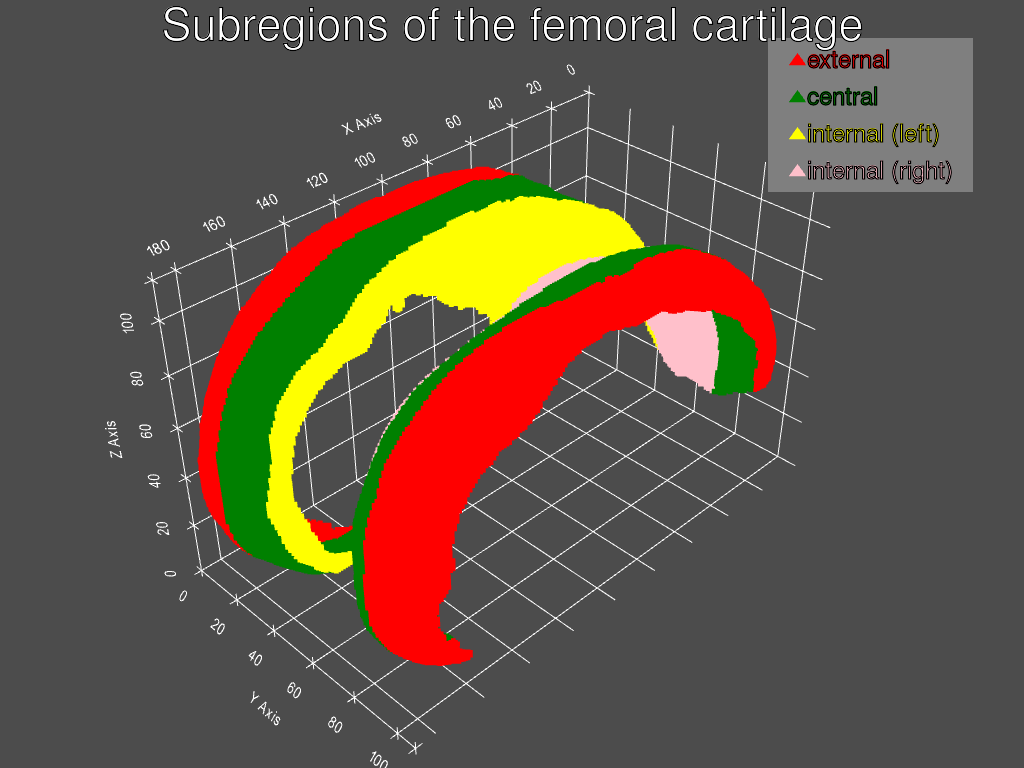
\includegraphics[width=\linewidth]{./figures/femoral_subregions}
	\caption{Subregions of the femoral cartilage}
	\label{fig:femoral_subregions}
\end{figure}

\begin{figure}[htb!]
	\centering
	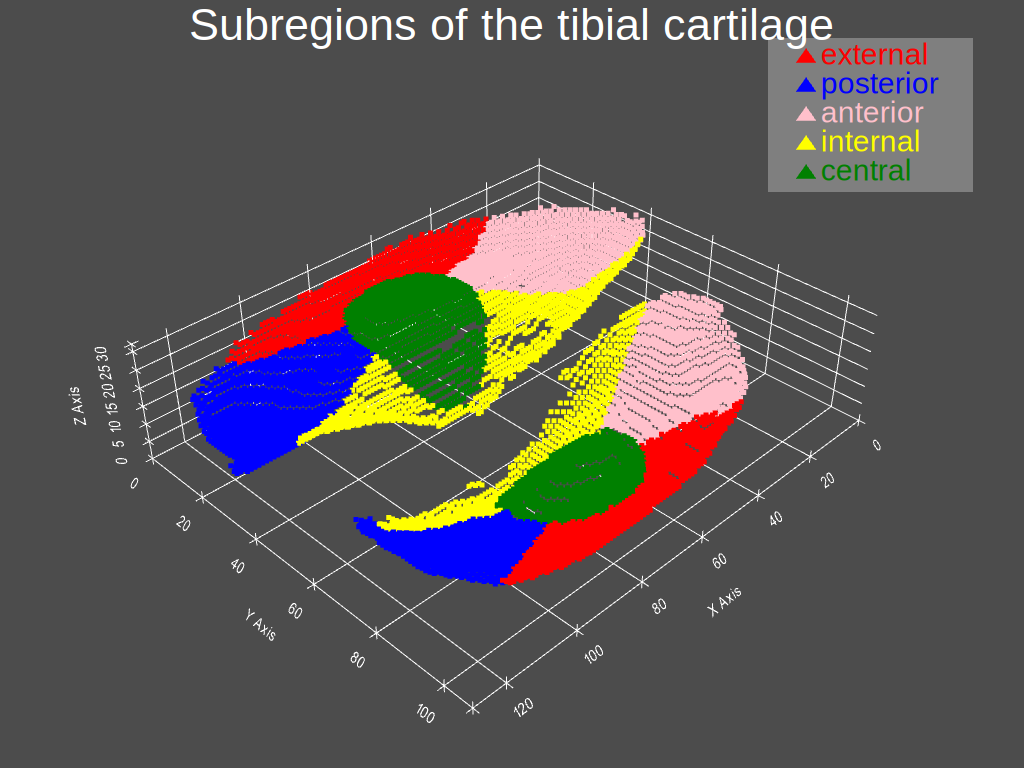
\includegraphics[width=\linewidth]{./figures/tibial_subregions}
	\caption{Subregions of the tibial cartilage}
	\label{fig:tibial_subregions}
\end{figure}